% SupplyGuard research paper (IEEEtran conference format).
% Compile from this folder (figures are in ./figures):  pdflatex SupplyGuard_Research_Paper.tex  (run twice)
% Every number comes from outputs/results and docs/paper/evidence (see EVIDENCE.md).
\documentclass[conference]{IEEEtran}

\usepackage{cite}
\usepackage{amsmath,amssymb}
\usepackage{graphicx}
\usepackage{booktabs}
\usepackage{array}
\usepackage{algorithm}
\usepackage[noend]{algpseudocode}
\usepackage{xcolor}
\usepackage[hidelinks]{hyperref}

\graphicspath{{figures/}}
\newcommand{\RI}{\mathrm{RI}}
\newcommand{\ReLU}{\mathrm{ReLU}}
\def\BibTeX{{\rm B\kern-.05em{\sc i\kern-.025em b}\kern-.08em T\kern-.1667em\lower.7ex\hbox{E}\kern-.125em X}}

\begin{document}

\title{SupplyGuard: A Temporal Graph Neural Network Framework for Predictive Supply Chain Disruption Risk Propagation}

\author{
\IEEEauthorblockN{Vemula Sanath Chandra}
\IEEEauthorblockA{Dept.\ of Computer Science and Engineering\\
Anurag University, Hyderabad, India\\
sanathchandra2005@gmail.com}
\and
\IEEEauthorblockN{Malyala Sai Bharadwaj}
\IEEEauthorblockA{Dept.\ of Computer Science and Engineering\\
Anurag University, Hyderabad, India\\
saimalyala7@gmail.com}
\and
\IEEEauthorblockN{Swami Sriharsha}
\IEEEauthorblockA{Dept.\ of Computer Science and Engineering\\
Anurag University, Hyderabad, India\\
sriharshaswamy@gmail.com}
\thanks{Under the guidance of Mrs.\ N.\ Chandana, Assistant Professor, Dept.\ of Computer Science and Engineering, Anurag University.}
}

\maketitle

\begin{abstract}
Multi-echelon supply networks can transmit an upstream disruption to downstream tiers, yet many risk-forecasting models predict a single aggregated index and are evaluated at very short horizons where persistence is difficult to beat. We present SupplyGuard, a spatio-temporal model that forecasts the risk indices of four echelons (Supplier, Manufacturer, Distributor, Retailer) ten minutes ahead ($H=5$ steps). It combines a two-layer relational graph convolution with separate upstream and downstream messages, a shared two-layer LSTM per node, and a residual head that predicts the change from the current state; Integrated Gradients provides post hoc, node-level attributions. On the Mendeley SCRM time-series dataset (592,599 usable rows after cleaning; chronological 80/10/10 split; 57,875 test windows), the directed model reduces the mean-node MSE to $2.73\times10^{-4}\pm0.03\times10^{-4}$ (five seeds), 31\% below Naive Persistence ($3.97\times10^{-4}$) and 4\% below a graph-free LSTM ($2.84\times10^{-4}$). The gain is concentrated on shock windows, where its error is about half that of persistence, while on calm windows it is about twice as large. Persistence remains the most accurate on three-tier severity classification (83.6\% vs 81.3\%). Integrated Gradients attributions have a median completeness gap of $9.4\times10^{-5}$ and describe local model sensitivity, not causal effects. Limitations include a confounded graph-free ablation and a single linear topology.
\end{abstract}

\begin{IEEEkeywords}
Supply chain networks, graph convolutional networks, spatio-temporal modeling, ripple effect propagation, LSTM recurrence, explainable artificial intelligence, path-integrated gradients, residual risk forecasting.
\end{IEEEkeywords}

%==================================================================================
\section{Introduction}
Contemporary manufacturing and commerce rely on lean inventory management, just-in-time (JIT) fulfillment and tightly synchronized transportation networks. These practices reduce holding costs in steady state but leave little buffer against disturbances. When an upstream tier is disrupted, for example by a production outage, component stockout or port congestion, the schedule deviation can propagate through intermediate facilities and distribution hubs and appear as stockouts at the retail tier. This propagation is studied in the supply chain literature as the ripple effect \cite{r1,r7}.

In response, operations teams increasingly use continuous telemetry of material transit, machine status, inventory levels and logistics cost. Converting such a stream into forecasts is typically done with autoregressive estimators, discrete-event simulators or Long Short-Term Memory (LSTM) networks \cite{r4}, and machine learning is being applied to supply chain management more broadly \cite{r12}. Two limitations of these formulations motivate this work.

First, many formulations, including the hybrid graph-LSTM model that we re-implement as a baseline \cite{r10}, predict a single aggregated index of network risk. An aggregate index does not show whether a bottleneck originates at a supplier or at a distributor, so corrective action cannot be targeted. Second, short-horizon forecasts are easy to match with a trivial baseline: in the dataset used here, adjacent two-minute observations are very strongly correlated (lag-1 Pearson $r$ between 0.97 and 0.996 across the four echelons), so predicting that the future equals the present is difficult to beat. A forecasting model must therefore be judged against persistence.

\subsection{Motivation}
\begin{itemize}
\item \textbf{Fragility of lean multi-tier chains:} Lean networks hold limited buffers, so a local supplier bottleneck can propagate to later echelons \cite{r1}.
\item \textbf{Limited visibility in aggregate indices:} A single network-wide index does not show which echelon is deteriorating.
\item \textbf{The 10-minute horizon:} Extending the forecast from 2 minutes ($H=1$) to 10 minutes ($H=5$) gives more lead time while remaining short enough to be compared directly with a persistence baseline.
\item \textbf{The need for interpretable output:} Operators need to know which inputs a forecast is sensitive to. Integrated Gradients gives signed, node-level sensitivities with a measurable completeness check, but these are not causal explanations.
\end{itemize}

\subsection{Objectives}
\begin{enumerate}
\item[\textbf{O1.}] Forecast the risk indices of the four echelons concurrently, ten minutes ($H=5$ steps) ahead, from a ten-step window.
\item[\textbf{O2.}] Represent directed material flow with a graph layer that treats upstream and downstream messages separately.
\item[\textbf{O3.}] Benchmark the model against Naive Persistence, Ridge-AR(10) and a graph-free LSTM under one chronological split and five seeds.
\item[\textbf{O4.}] Attach Integrated Gradients attributions to each forecast and report their completeness gap and a deletion test.
\item[\textbf{O5.}] State where the learned model adds value over persistence and where it does not.
\end{enumerate}

\subsection{Key Methodological Contributions}
\begin{itemize}
\item \textbf{Directed spatio-temporal architecture:} A relational graph convolution with separate self, upstream and downstream weights is applied at every time step, followed by a shared LSTM per node (Section~\ref{sec:math}).
\item \textbf{Concurrent node-level forecasts:} A single forward pass gives the four echelon forecasts, from which the mean risk index is derived.
\item \textbf{Residual persistence anchoring:} The head predicts the change from the current state, so the model starts from the persistence forecast \cite{r18}.
\item \textbf{Evaluation against persistence:} Five-seed results with standard deviations against Naive Persistence, Ridge-AR(10) and a graph-free LSTM, reported separately for shock and calm windows, plus a measured completeness check for Integrated Gradients \cite{r8}.
\end{itemize}

\subsection{Problem Statement and Formal Framing}
We represent the multi-echelon supply network as a directed graph $G=(V,E)$, where $|V|=4$ nodes are the Tier-1 Supplier (S), Manufacturer (M), Regional Distributor (D) and Final Retailer (R), and $E=\{(S,M),(M,D),(D,R)\}$ is the direction of material flow. At each time step $t$ the system observes $x_t\in\mathbb{R}^{5}$: the min--max scaled risk indices of the four echelons and the concurrent Total Cost. Given a lookback window of $L=10$ consecutive observations, the input is $X\in\mathbb{R}^{L\times5}$. The task is to learn a mapping $f_\theta$ from $X$ to the risk vector $\hat{y}_{t+H}\in\mathbb{R}^{4}$ at horizon $H=5$ steps (nominally 10 minutes), and, for a chosen target node $k$, to compute an attribution matrix $\mathrm{Attr}\in\mathbb{R}^{L\times5}$ that measures the local sensitivity of the forecast of node $k$ to each past input.

%==================================================================================
\section{Literature Survey}
\subsection{Disruption Cascades and Ripple Effect Modeling}
Ripple-effect research has been studied through analytical and simulation lenses. Ivanov, Dolgui and Sokolov \cite{r1} analysed how digital technology and Industry~4.0 affect ripple-effect and supply chain risk analytics. Dolgui, Ivanov and Sokolov \cite{r7} reviewed quantitative ripple-effect research, separating it from the bullwhip effect and grouping the approaches into optimisation, simulation, control-theoretic and reliability methods. Simchi-Levi et al.\ \cite{r2} describe Time-to-Survive (TTS) and Time-to-Recover (TTR) as measures of how long a network can keep operating, and how long recovery takes, when a node fails.

\subsection{Sequence Learning and Graph Neural Architectures}
To handle high-frequency telemetry, researchers adopted recurrent networks. Hochreiter and Schmidhuber \cite{r4} introduced the Long Short-Term Memory (LSTM) network, which mitigates vanishing gradients over long sequences. A plain LSTM over the stacked input does not encode which facility supplies which. Scarselli et al.\ \cite{r16} introduced the graph neural network model, and Kipf and Welling \cite{r6} simplified it to the Graph Convolutional Network (GCN) for semi-supervised node classification. Yu, Yin and Zhu \cite{r5} combined spatial graph convolutions with temporal convolutions for traffic forecasting (STGCN), and Li et al.\ \cite{r17} modelled traffic as diffusion on a directed graph inside a recurrent network. Wu et al.\ \cite{r9} survey graph neural networks, and Veli\v{c}kovi\'c et al.\ \cite{r13} introduced graph attention networks.

Farzhana and Dev Harris \cite{r10} fuse a graph convolution with an LSTM to predict supply chain risk on the same dataset used here. We re-implement that fusion as a baseline (global mean pooling of the graph output to a scalar risk index) and extend it to node-level forecasting; the pooling and layer sizes of our re-implementation are our interpretation of the published description, not a verbatim specification.

\subsection{Explainability}
Attribution methods require care. Adebayo et al.\ \cite{r15} showed that several saliency methods can produce maps that are insensitive to the model's parameters or to the data labels, which motivates sanity checks for any attribution. Sundararajan, Taly and Yan \cite{r8} proposed Integrated Gradients (IG), which accumulates gradients along a straight path from a baseline and satisfies Sensitivity and Implementation Invariance; completeness (the attributions sum to the difference in model output) follows. Lundberg and Lee \cite{r19} unify additive feature-attribution methods, an alternative that we do not use. We apply IG to the directed graph model and report its completeness gap and a deletion test.

\begin{table}[t]
\caption{Summary of Prior Approaches and Methodological Limits}
\label{tab:prior}
\centering
\footnotesize
\begin{tabular}{@{}p{0.7cm}p{0.7cm}p{2.0cm}p{1.6cm}p{2.2cm}@{}}
\toprule
Ref. & Year & Methodology & Scope & Key limitation \\
\midrule
\cite{r7}  & 2018 & Literature review (optimisation, simulation, control, reliability) & Ripple-effect research & Review; no learned telemetry forecaster \\
\cite{r2}  & 2014 & Time-to-Survive / Time-to-Recover analysis & Supplier mapping & Analytical; not designed for minute-level telemetry \\
\cite{r10} & 2025 & Hybrid GNN-LSTM & Mendeley SCRM telemetry & Re-implemented here with a scalar risk output \\
\cite{r5}  & 2018 & Spatio-temporal graph convolution & Road sensor networks & Traffic forecasting; not evaluated on supply chains \\
\cite{r8}  & 2017 & Integrated Gradients & Image, text and other models & Needs a scalar target and a chosen baseline \\
\cite{r17} & 2018 & Diffusion convolutional recurrent network & Traffic forecasting & Directed diffusion on road graphs; not applied to supply chains \\
\bottomrule
\end{tabular}
\end{table}

\subsection{Research Gap}
The work reviewed above leaves three gaps that this paper addresses. First, the hybrid GNN-LSTM for this dataset \cite{r10} outputs one aggregated risk index, so the affected echelon is not identified. Second, spatio-temporal graph models such as \cite{r5} are built for symmetric road networks, while material flow in a supply chain is directed; we therefore compare a symmetric (Kipf--Welling \cite{r6}) and a directed variant. Third, forecasts should be reported against persistence, which is strong at short horizons. We do not claim that attribution identifies a root cause.

%==================================================================================
\section{Proposed Methodology and Implementation}
\subsection{System Architecture and Pipeline Overview}
SupplyGuard has five stages, shown in Fig.~\ref{fig:arch} and Fig.~\ref{fig:pipe}: cleaning and windowing of the telemetry, two graph-convolution layers applied at every time step, a shared LSTM per node, a residual head that forecasts the four risk indices five steps (nominally ten minutes) ahead, and post hoc Integrated Gradients attribution.

\begin{figure}[t]
\centering
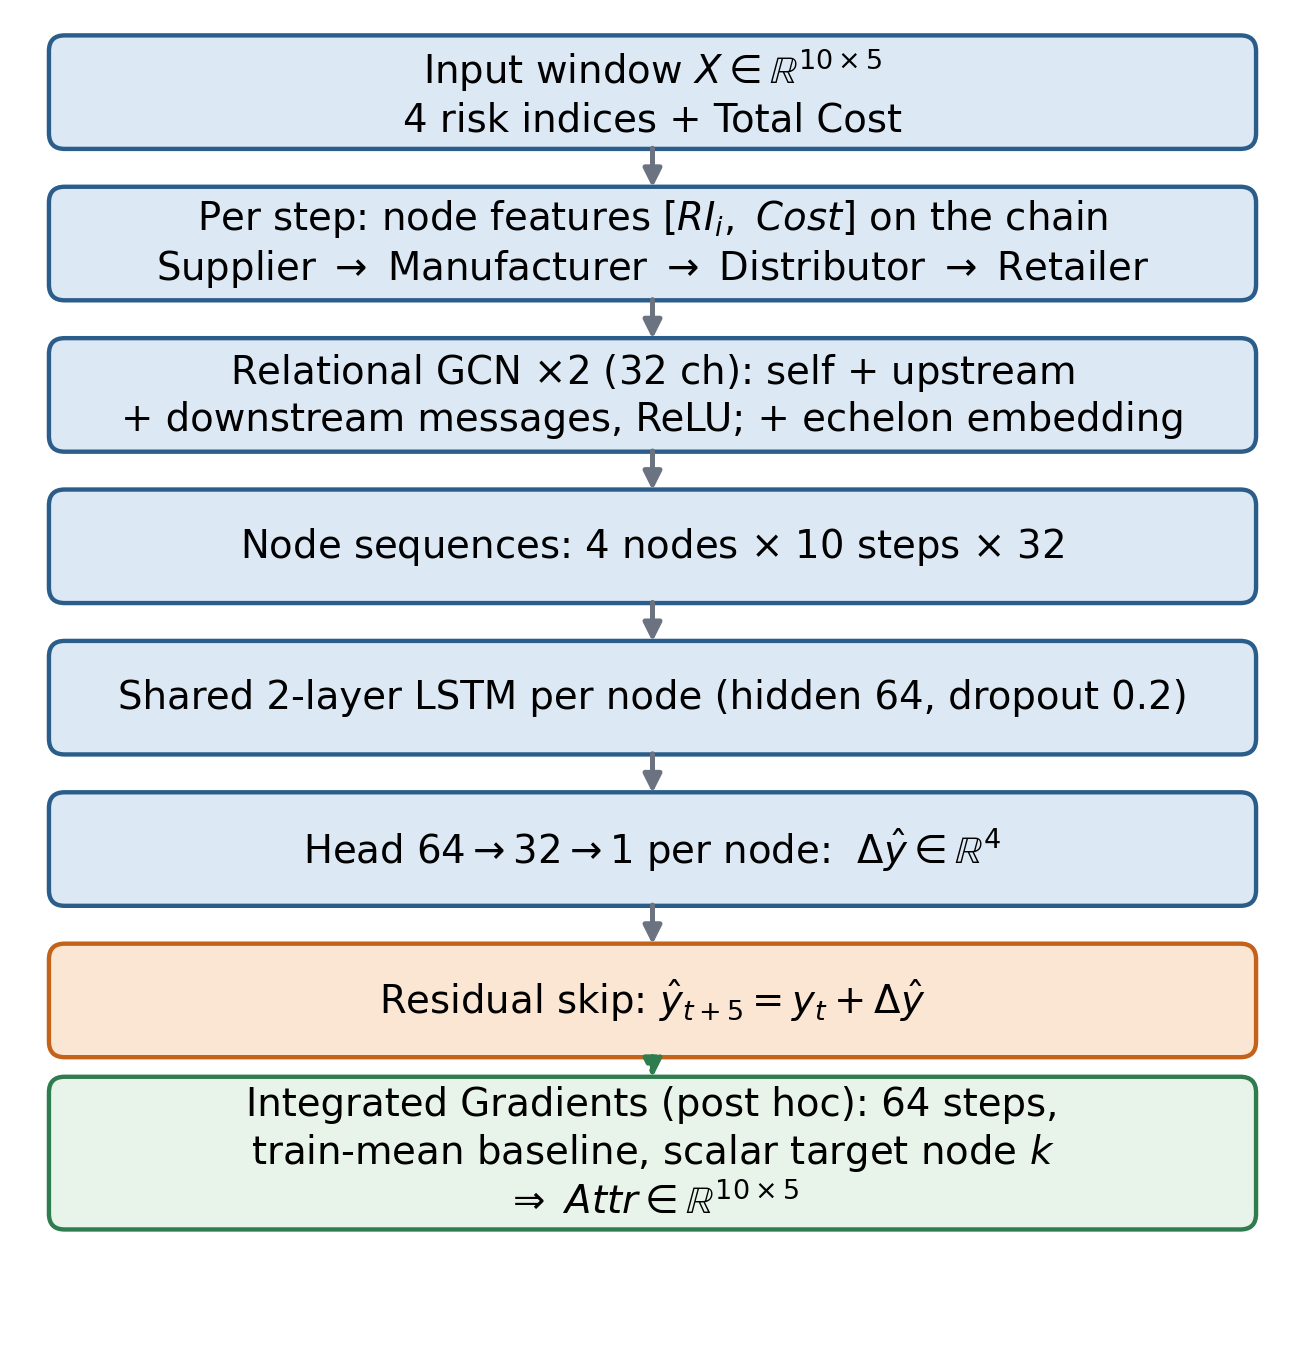
\includegraphics[width=\columnwidth]{fig1.png}
\caption{SupplyGuard model: two relational graph-convolution layers with self, upstream and downstream messages, a shared per-node LSTM, a residual head, and the Integrated Gradients module.}
\label{fig:arch}
\end{figure}

\begin{figure}[t]
\centering
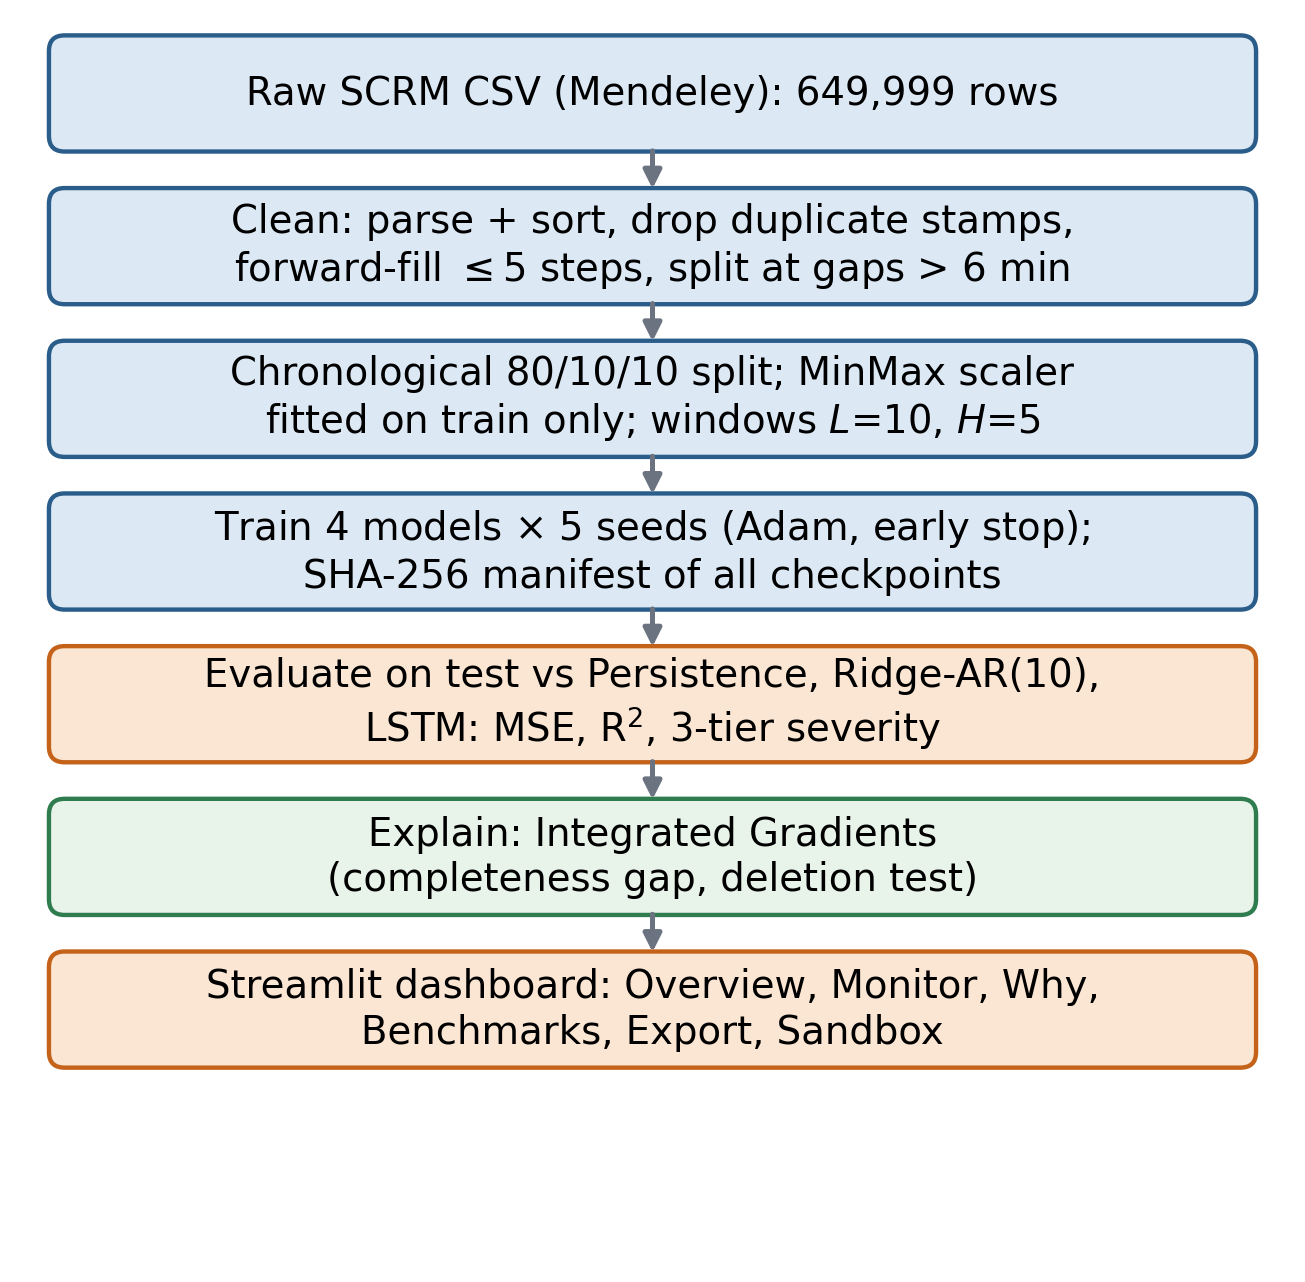
\includegraphics[width=\columnwidth]{fig2.png}
\caption{Processing pipeline: cleaning, chronological split with train-only scaling, five-seed training, evaluation against baselines, Integrated Gradients, and the Streamlit dashboard.}
\label{fig:pipe}
\end{figure}

\subsection{Software Engineering and Component Architecture}
Figure~\ref{fig:modules} shows the module structure of the implementation. \texttt{src/dataset.py} builds leakage-safe windows (chronological split; scaler fitted on the training partition only), \texttt{src/graph\_builder.py} builds the symmetric and directed adjacency matrices, and \texttt{src/models/graph\_layers.py} implements the graph convolution natively in PyTorch (no PyTorch Geometric). \texttt{src/models/st\_gcn\_lstm.py} defines the proposed model and the neural baselines, \texttt{training/} trains and evaluates them, \texttt{src/explainability.py} implements Integrated Gradients, and a Streamlit application reads the saved outputs.

\begin{figure}[t]
\centering
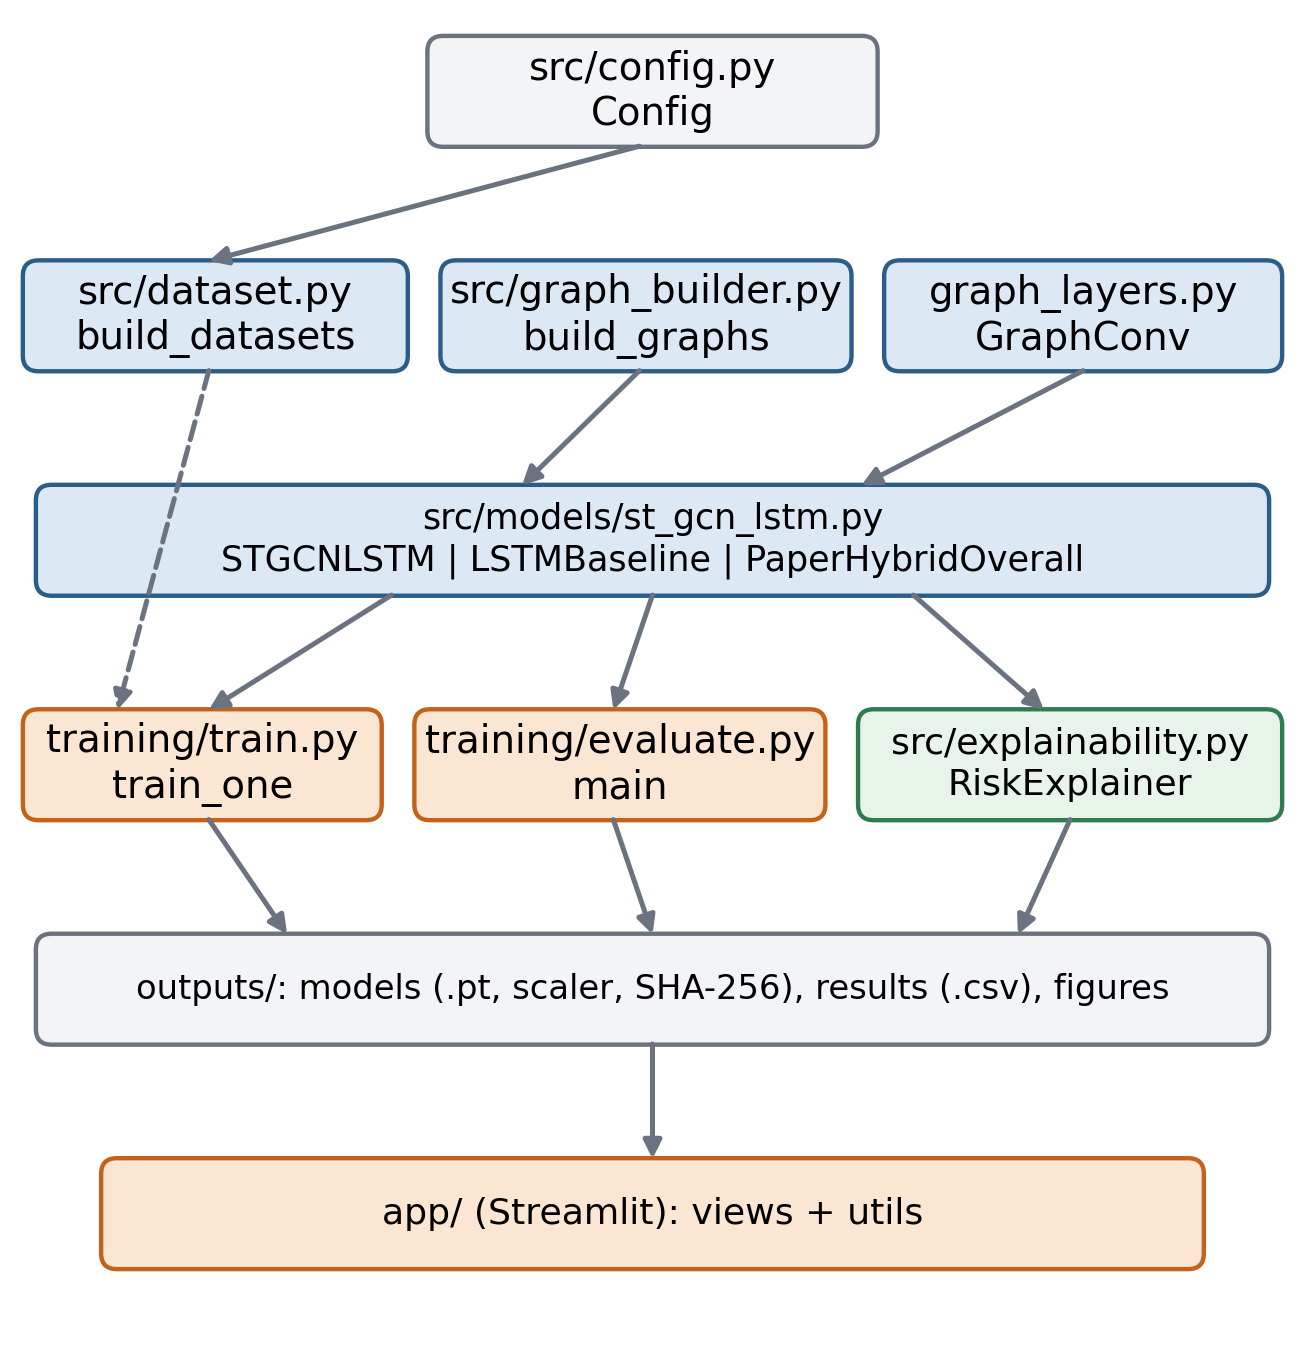
\includegraphics[width=\columnwidth]{fig3.png}
\caption{Module dependencies of the implementation (\texttt{src/}, \texttt{training/}, \texttt{app/}).}
\label{fig:modules}
\end{figure}

\subsection{Dataset Provenance and Preprocessing Protocol}
We use the Mendeley time-series dataset for risk assessment in supply chain networks \cite{r3} (file \texttt{SCRM\_timeSeries\_2018\_train.csv}). It has 649,999 rows between 28 Jan 2015 and 19 Dec 2018, with records for 2015, 2016 and 2018 only. Each row holds a timestamp, the risk index of each of the four echelons and Total Cost, nominally every two minutes. Cleaning removes 2,363 duplicate timestamps, forward-fills gaps of at most five steps, drops 53,960 rows that remain incomplete and 1,077 rows in segments shorter than 15 steps, and splits sequences wherever the time gap exceeds six minutes. This leaves 592,599 rows (91.2\%). The cleaned rows are split chronologically 80/10/10 (474,079 / 59,259 / 59,261 rows). A window of $L=10$ rows predicts the risk indices five rows later, and windows never cross a segment boundary, so every target lies inside its own partition; this gives 460,135 training, 57,817 validation and 57,875 test windows, with the test windows spanning 17 Sep to 19 Dec 2018. Because windows are indexed by rows, the horizon is five rows; its median duration is 10.0 minutes and its mean 10.8 minutes. The min--max scaler is fitted on the training partition only. Before cleaning, 5.1\% of Distributor values and 5.5\% of Total Cost values are missing.

\begin{table}[t]
\caption{Mendeley SCRM Telemetry Channels and Training-Partition Statistics (Raw Units)}
\label{tab:data}
\centering
\footnotesize
\begin{tabular}{@{}llccc@{}}
\toprule
Echelon & Node & Channel & Mean & Std \\
\midrule
Tier-1 Supplier & S & \texttt{RI\_Supplier1} & 1.701 & 0.041 \\
Manufacturer & M & \texttt{RI\_Manufacturer1} & 2.711 & 1.134 \\
Regional Distributor & D & \texttt{RI\_Distributor1} & 2.452 & 0.705 \\
Final Retailer & R & \texttt{RI\_Retailer1} & 2.413 & 0.252 \\
Logistics network & -- & \texttt{Total\_Cost} & 87.606 & 76.607 \\
\bottomrule
\end{tabular}
\end{table}

\subsection{Mathematical Model Formulation}\label{sec:math}
\subsubsection{Relational graph convolution}
Let $A\in\{0,1\}^{4\times4}$ with $A_{i,j}=1$ if facility $i$ ships to facility $j$ (edges S$\to$M, M$\to$D, D$\to$R). We define $A_{\mathrm{down}}=\mathrm{rownorm}(A^{\top})$, which averages messages from upstream parents, and $A_{\mathrm{up}}=\mathrm{rownorm}(A)$, which averages messages from downstream children. At each time step the node features $H^{(0)}\in\mathbb{R}^{4\times2}$ hold each node's risk index and the Total Cost. Each layer computes
\begin{equation}
H^{(l+1)}=\ReLU\!\big(H^{(l)}W^{(l)}_{\mathrm{self}}+A_{\mathrm{down}}H^{(l)}W^{(l)}_{\mathrm{down}}+A_{\mathrm{up}}H^{(l)}W^{(l)}_{\mathrm{up}}+b^{(l)}\big),
\end{equation}
where $W_{\mathrm{self}},W_{\mathrm{down}},W_{\mathrm{up}}\in\mathbb{R}^{F_{\mathrm{in}}\times F_{\mathrm{out}}}$ are learnable, $b$ is a bias and $F_{\mathrm{out}}=32$. Two layers are stacked so that information can travel two hops (S can influence D). A learnable echelon embedding is added to the output, $H^{(2)}\in\mathbb{R}^{4\times32}$. The symmetric variant uses $\ReLU(\hat{A}HW+b)$ with $\hat{A}=\tilde{D}^{-1/2}(A_{\mathrm{sym}}+I)\tilde{D}^{-1/2}$ \cite{r6}.

\subsubsection{Recurrent temporal memory}
For each node the $L=10$ embeddings form a sequence in $\mathbb{R}^{10\times32}$. A two-layer LSTM (hidden size 64, dropout 0.2) with weights shared across the four nodes maps each node's sequence to its final hidden state:
\begin{equation}
h^{(i)}_t=\mathrm{LSTM}\big(H^{(2)}_{\tau,i}:\tau=t-L+1,\dots,t\big),
\end{equation}
with $h^{(i)}_t\in\mathbb{R}^{64}$. Total Cost enters through the node features; it is not concatenated again after the graph layers.

\subsubsection{Residual persistence head}
A perceptron ($64\to32\to1$, ReLU, dropout 0.2) maps $h^{(i)}_t$ to a correction, and the forecast adds it to the current value \cite{r18}:
\begin{equation}
\hat{y}^{(i)}_{t+H}=x^{(i)}_t+g\big(h^{(i)}_t\big).
\end{equation}
With a zero correction the model reproduces persistence, so any gain must come from the learned correction.

\subsubsection{Training objective}
The four echelons are predicted jointly, a form of multi-task learning \cite{r14}, by minimising the mean squared error. No explicit weight decay is used; early stopping on validation loss is the regulariser.
\begin{equation}
\mathcal{L}(\theta)=\frac{1}{|V|}\sum_{i=1}^{|V|}\big(\hat{y}^{(i)}_{t+H}-y^{(i)}_{t+H}\big)^2 .
\end{equation}

\subsubsection{Integrated Gradients}
For a window $X$ and a target node $k$, the scalar output is $f_k(X)=\hat{y}^{(k)}_{t+H}$. With baseline $X^{(0)}$ (the training-mean feature vector repeated over the window) and $M=64$ steps, the attribution is
\begin{equation}
\mathrm{Attr}(X)=\big(X-X^{(0)}\big)\odot\frac{1}{M}\sum_{m=1}^{M}\left.\frac{\partial f_k}{\partial X}\right|_{X^{(0)}+\frac{m}{M}(X-X^{(0)})}.
\end{equation}
Completeness requires $\sum\mathrm{Attr}=f_k(X)-f_k(X^{(0)})$; we report the residual. Attributions describe local sensitivity along this path and are not causal effects.

\begin{algorithm}[t]
\caption{SupplyGuard Forecasting and Attribution}
\label{alg:sg}
\begin{algorithmic}[1]
\small
\Require window $X\in\mathbb{R}^{L\times5}$ (columns 1--4 risk indices, column 5 Total Cost), $L=10$, $H=5$; $A_{\mathrm{down}},A_{\mathrm{up}}$; target node $k$; $M=64$; baseline $X^{(0)}$
\Ensure forecast $\hat{y}_{t+H}\in\mathbb{R}^4$; attribution $\mathrm{Attr}\in\mathbb{R}^{L\times5}$; completeness gap
\For{$\tau=t-L+1$ \textbf{to} $t$}
  \State $S_\tau\gets$ per-node features $[x_\tau[i],x_\tau[5]]\in\mathbb{R}^{4\times2}$
  \State $H^1\gets\ReLU(S_\tau W^0_{\mathrm{self}}+A_{\mathrm{down}}S_\tau W^0_{\mathrm{down}}+A_{\mathrm{up}}S_\tau W^0_{\mathrm{up}}+b^0)$
  \State $H^2\gets\ReLU(H^1W^1_{\mathrm{self}}+A_{\mathrm{down}}H^1W^1_{\mathrm{down}}+A_{\mathrm{up}}H^1W^1_{\mathrm{up}}+b^1)+E$
\EndFor
\For{each node $i$} \Comment{LSTM weights shared across nodes}
  \State $h^{(i)}\gets\mathrm{LSTM}(H^2_{t-L+1,i},\dots,H^2_{t,i})\in\mathbb{R}^{64}$
  \State $\hat{y}^{(i)}_{t+H}\gets x_t[i]+g(h^{(i)})$
\EndFor
\State \textit{// post hoc attribution for target node $k$}
\State $X^{(0)}\gets$ training-mean window
\For{$m=1$ \textbf{to} $M$}
  \State $X^{(m)}\gets X^{(0)}+\frac{m}{M}(X-X^{(0)})$
  \State $G^{(m)}\gets\partial\hat{y}^{(k)}_{t+H}/\partial X^{(m)}$
\EndFor
\State $\mathrm{Attr}\gets(X-X^{(0)})\odot\frac{1}{M}\sum_m G^{(m)}$
\State $\mathrm{gap}\gets\big|\sum\mathrm{Attr}-(\hat{y}^{(k)}(X)-\hat{y}^{(k)}(X^{(0)}))\big|$
\State \Return $\hat{y}_{t+H},\mathrm{Attr},\mathrm{gap}$
\end{algorithmic}
\end{algorithm}

\subsection{Training Configuration and Hyperparameters}
The model is implemented in PyTorch; the graph layers are written natively (no PyTorch Geometric). The four neural models (LSTM, ST-GCN symmetric, ST-GCN directed and the scalar paper-style hybrid) were trained with five seeds (42--46) in a Google Colab session on an NVIDIA A100 GPU (40~GB), batch size 256, with Adam \cite{r20} (learning rate $10^{-3}$, no weight decay), gradient-norm clipping at 1.0, at most 50 epochs and early stopping with patience 10 on validation loss. Training took 140--638~s per run. Reported metrics are means $\pm$ sample standard deviation over the five seeds; Persistence and Ridge-AR(10) are deterministic. Inference and attribution timings in Tables~\ref{tab:hyper} and~\ref{tab:ig} were measured on a CPU (PyTorch 2.12, four threads) and vary from run to run.

\begin{table}[t]
\caption{Hyperparameters and Measured Timings}
\label{tab:hyper}
\centering
\footnotesize
\begin{tabular}{@{}p{2.4cm}p{2.5cm}p{2.5cm}@{}}
\toprule
Parameter & Value & Note \\
\midrule
Lookback window $L$ & 10 steps (20 min nominal) & Window length for every model \\
Horizon $H$ & 5 rows (nominal 10 min) & Median 10.0 min, mean 10.8 min in the cleaned data \\
Graph layers & 2 layers, 32 channels & Two hops let the supplier reach the distributor \\
LSTM (ST-GCN models) & 2 layers, hidden 64, dropout 0.2 & Weights shared across the four nodes \\
Adam learning rate / weight decay & $10^{-3}$ / none & Early stopping, patience 10 \\
IG steps $M$ & 64 & Gap reported in Table~\ref{tab:ig} \\
Inference latency (CPU, batch 1) & about 2.5 ms & Measured; varies between runs \\
\bottomrule
\end{tabular}
\end{table}

\subsection{Continuous and Categorical Evaluation Criteria}
For continuous tracking we report MSE, MAE, RMSE and $R^2$ on the mean of the four echelon forecasts (derived 4-node mean), plus per-node MSE and the skill relative to persistence, $1-\mathrm{MSE}/\mathrm{MSE}_{\mathrm{persistence}}$. For alert-style evaluation, each node's value is assigned to a Low, Medium or High tier using that node's training-set terciles, and accuracy and macro-F1 are computed over all node-window pairs. The test tiers are not balanced (Low 54,065, Medium 86,290, High 91,145 pairs), and for the Supplier the two thresholds differ by only 0.003 in scaled units. We also report error separately on shock windows (the top 5\% of windows by mean $|y(t+H)-y(t)|$; 2,894 windows) and on the remaining calm windows.

%==================================================================================
\section{Results Analysis and Experimental Benchmarks}
\subsection{Baseline Comparison Architectures}
We compare against: (1) Naive Persistence, $\hat{y}_{t+H}=x_t$; (2) Ridge-AR(10), ridge regression \cite{r11} on the 50 flattened lookback features with the penalty tuned on the validation set ($\alpha=10$); (3) a graph-free LSTM, a two-layer LSTM over the five input features with a joint four-output head and the same residual connection, trained for five seeds; and (4) a scalar paper-style GCN--LSTM hybrid re-implementing \cite{r10}, which predicts only the mean risk index and is therefore not in Table~\ref{tab:main}. The LSTM and the ST-GCN differ in more than the graph (a joint head versus a shared per-node LSTM), so the comparison is not a pure test of message passing.

\subsection{Quantitative Benchmark Findings}
Table~\ref{tab:main} reports test results on 57,875 windows at $H=5$. The directed model has the lowest MSE ($2.73\times10^{-4}\pm0.03\times10^{-4}$), $31.2\%\pm0.7\%$ below Naive Persistence and 3.8\% below the LSTM ($2.84\times10^{-4}$). The gap to the LSTM ($0.11\times10^{-4}$) exceeds the sum of the two standard deviations ($0.06\times10^{-4}$), the criterion we use for claiming an improvement, but the LSTM has a slightly lower MAE and the architectures differ, so we do not attribute the gap to graph structure alone. The symmetric variant is worse and less stable ($3.30\times10^{-4}\pm0.61\times10^{-4}$); two of its five seeds stopped at the persistence solution during training. Ridge-AR(10) improves on persistence by 10.8\%. On three-tier severity, Naive Persistence is the most accurate (83.6\% accuracy, 84.3\% macro-F1); no learned model exceeds it and the directed model is lower ($81.3\%\pm2.4\%$).

\begin{table*}[t]
\caption{Test Performance on 57,875 Windows ($H=5$, Mean of Four Nodes; Mean $\pm$ Std over 5 Seeds)}
\label{tab:main}
\centering
\footnotesize
\begin{tabular}{@{}lcccccc@{}}
\toprule
Architecture & MSE ($10^{-4}$) & MAE ($10^{-3}$) & RMSE ($10^{-2}$) & $R^2$ & Accuracy (\%) & Macro-F1 (\%) \\
\midrule
Naive Persistence & 3.97 & 5.493 & 1.992 & 0.9613 & 83.6 & 84.3 \\
Ridge-AR(10) & 3.54 & 6.351 & 1.881 & 0.9655 & 79.4 & 79.9 \\
Graph-free LSTM & $2.84\pm0.03$ & $5.118\pm0.093$ & $1.684\pm0.010$ & $0.9723\pm0.0003$ & $80.5\pm1.6$ & $81.1\pm1.6$ \\
ST-GCN-LSTM (symmetric) & $3.30\pm0.61$ & $5.385\pm0.147$ & $1.811\pm0.165$ & $0.9678\pm0.0059$ & $81.9\pm1.8$ & $82.5\pm2.0$ \\
ST-GCN-LSTM (directed), SupplyGuard & $\mathbf{2.73\pm0.03}$ & $5.238\pm0.259$ & $\mathbf{1.652\pm0.008}$ & $\mathbf{0.9734\pm0.0003}$ & $81.3\pm2.4$ & $81.9\pm2.5$ \\
\bottomrule
\end{tabular}
\end{table*}

\begin{figure}[t]
\centering
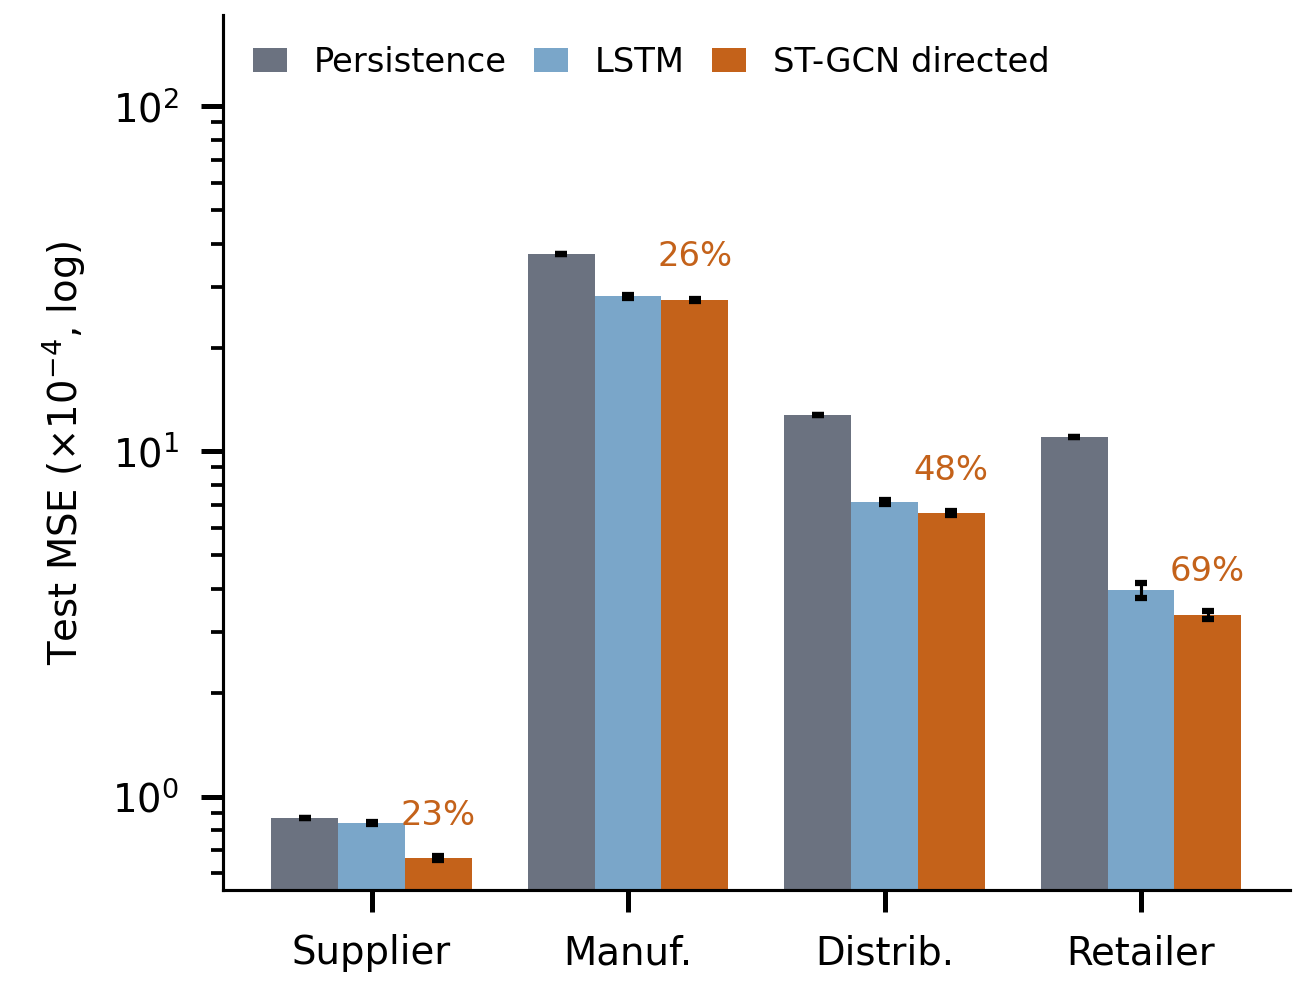
\includegraphics[width=\columnwidth]{fig4.png}
\caption{Per-echelon test MSE (log scale, mean $\pm$ std over five seeds); percentages are the directed model's MSE reduction relative to persistence.}
\label{fig:node}
\end{figure}

\subsection{Continuous Trajectory Tracking Dynamics}
Figure~\ref{fig:traj} shows 80 consecutive test windows around the largest Retailer shock in the test set. Persistence repeats the current value and therefore lags an abrupt change by about the forecast horizon. The directed model (five-seed mean) reacts earlier than persistence in the Retailer series, but it does not reproduce the step itself, and for the Distributor it produces a short overshoot at the onset. This is a single selected window, shown for illustration. Across the 2,894 shock windows the per-node MSE averaged over the four echelons is 0.0287 for persistence and 0.0146--0.0148 for the directed model (five seeds), about half; on the remaining calm windows persistence is better ($1.2\times10^{-4}$ versus $2.2$--$2.5\times10^{-4}$).

\begin{figure}[t]
\centering
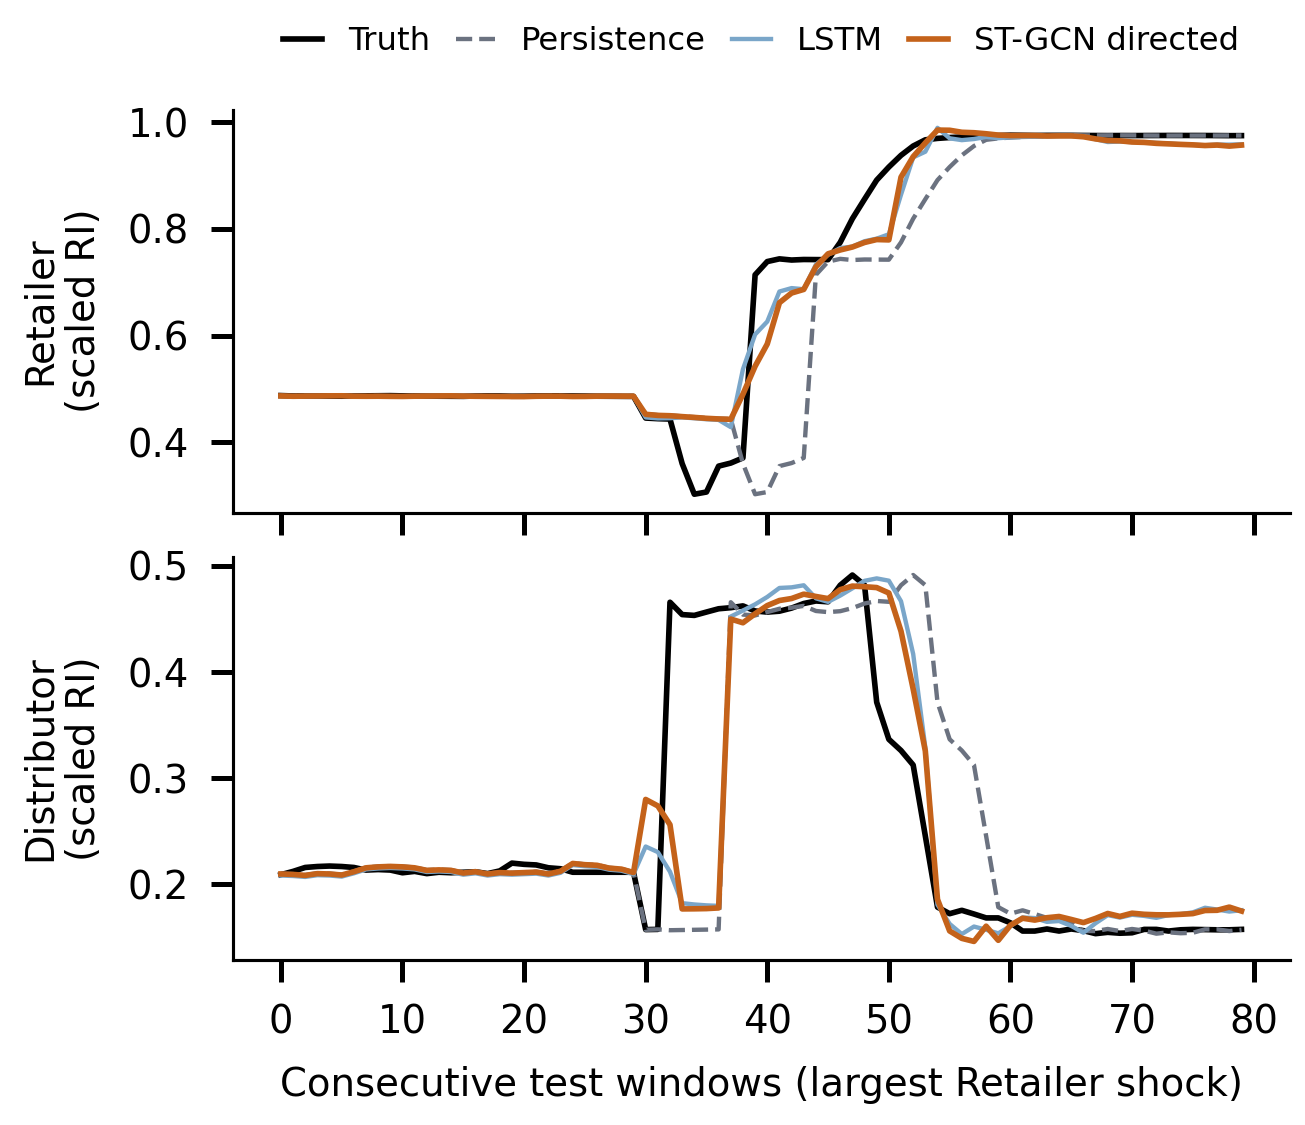
\includegraphics[width=\columnwidth]{fig5.png}
\caption{Truth, Persistence, LSTM and directed ST-GCN-LSTM (five-seed means) for the Retailer and the Distributor around the largest Retailer shock in the test set.}
\label{fig:traj}
\end{figure}

\subsection{Disruption Severity Classification and Alert Fidelity}
Figure~\ref{fig:cm} shows the three-tier confusion matrix of the directed model (seed 42) over 231,500 node-window pairs. Row-normalised recall is 89.4\% (Low), 82.6\% (Medium) and 82.5\% (High), and accuracy is 84.1\% for this seed (five-seed mean $81.3\%\pm2.4\%$). Errors occur mainly between adjacent tiers: 10,314 Medium cases are predicted High and 15,460 High cases are predicted Medium.

\begin{figure}[t]
\centering
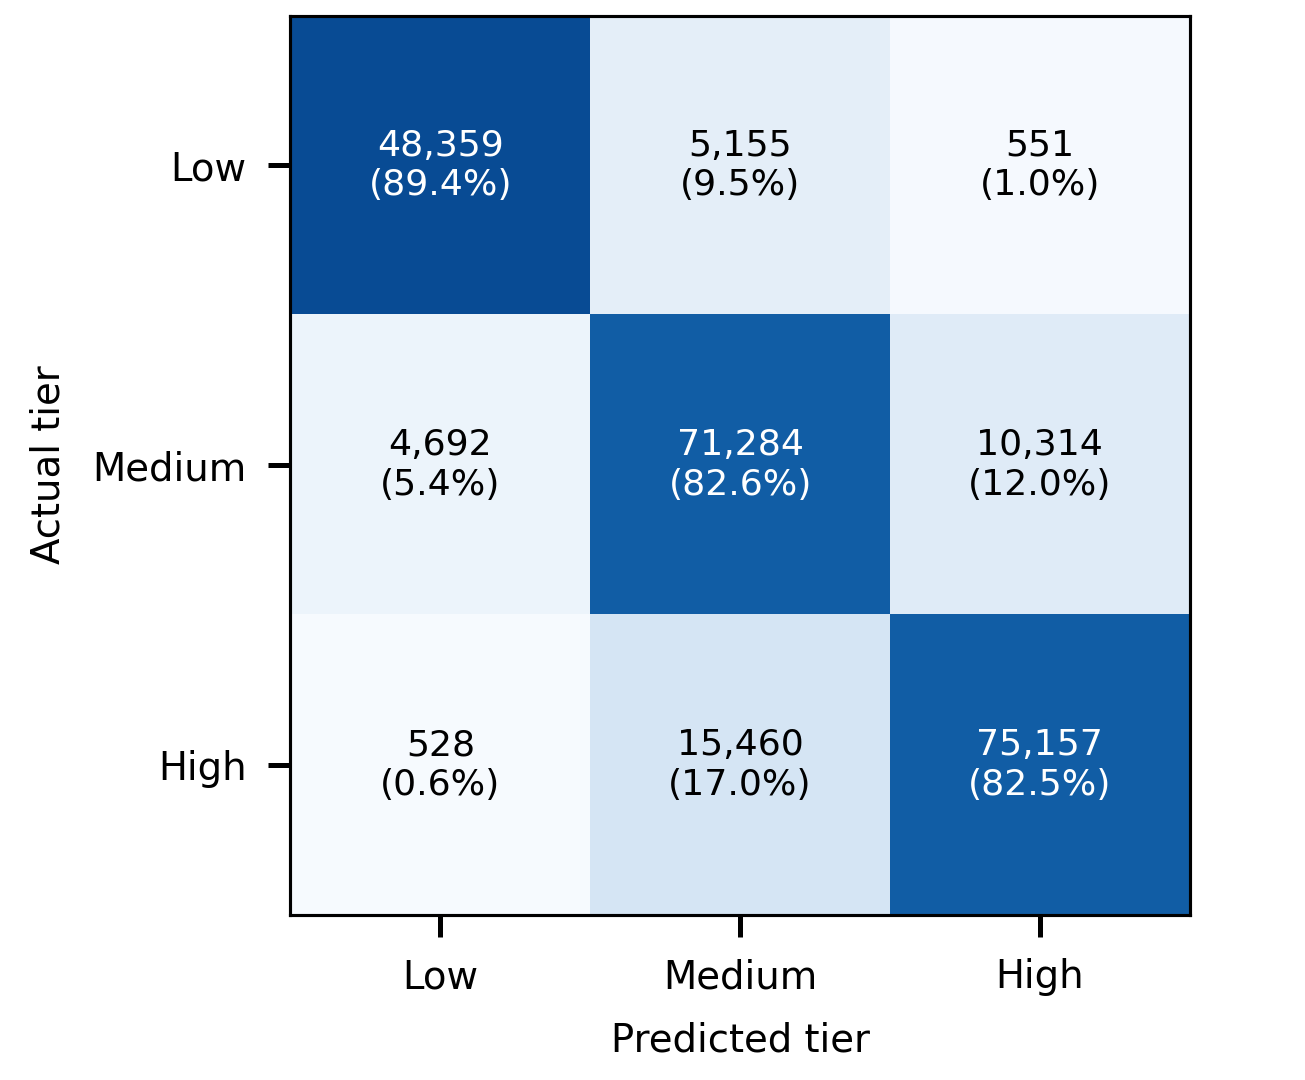
\includegraphics[width=\columnwidth]{fig6.png}
\caption{Three-tier severity confusion matrix of the directed ST-GCN-LSTM (seed 42): counts and row-normalised shares.}
\label{fig:cm}
\end{figure}

\begin{table}[t]
\caption{Per-Node Test MSE ($10^{-4}$) and Skill Relative to Persistence (Mean $\pm$ Std over 5 Seeds)}
\label{tab:node}
\centering
\footnotesize
\begin{tabular}{@{}lcccc@{}}
\toprule
Node & Persistence & LSTM & ST-GCN-Dir & Dir.\ skill (\%) \\
\midrule
Tier-1 Supplier (S) & 0.87 & $0.84\pm0.01$ & $0.66\pm0.01$ & 23.4 \\
Manufacturer (M) & 37.39 & $28.11\pm0.27$ & $27.49\pm0.19$ & 26.5 \\
Regional Distributor (D) & 12.76 & $7.14\pm0.12$ & $6.63\pm0.09$ & 48.0 \\
Final Retailer (R) & 10.98 & $3.96\pm0.20$ & $3.37\pm0.09$ & 69.3 \\
\midrule
Mean of the four nodes & 15.50 & 10.01 & 9.54 & 38.5 \\
\bottomrule
\end{tabular}
\end{table}

%==================================================================================
\section{Operational Discussion, Explainability and Ablation Insights}
\subsection{How Much Does the Model Add Over Persistence?}
Persistence is a strong baseline here: $R^2$ is 0.961 for the mean risk index and adjacent observations are correlated at $r=0.97$--$0.996$. The learned models nonetheless reduce the MSE by 28--31\%. The reduction is not uniform: it is largest for the Retailer (69\%) and the Distributor (48\%) and smaller for the Supplier (23\%) and the Manufacturer (26\%). It comes from shock windows, where the error is about half of persistence's; on calm windows the learned correction roughly doubles the error. A practical system might therefore use persistence in calm periods and the learned forecast when a change is detected; we have not tested such a hybrid. The graph-free LSTM reaches most of the gain (28.5\% versus 31.2\%). The directed model's MSE is below the LSTM's by more than the sum of the two seed standard deviations at every node; the largest relative difference is at the Supplier ($0.84\times10^{-4}$ versus $0.66\times10^{-4}$). Because the architectures differ in more than the graph, we regard graph structure as promising rather than proven.

\subsection{Integrated Gradients Attribution}
Figure~\ref{fig:ig} summarises attribution shares for each target node, as magnitude-weighted shares of $|\mathrm{attribution}|$ over 100 evenly spaced test windows and five seeds. In the forecast, a node's own current risk index dominates (53--74\%), followed by Total Cost (18--37\%); upstream echelons contribute little (the Supplier contributes 0.9\% to the Distributor forecast and essentially 0\% to the Retailer forecast). This largely reflects the residual connection, which copies each node's own current value into its forecast. Attributing only the learned correction shifts weight to Total Cost (37--55\%); for the Supplier and Retailer targets the correction is exactly zero in 73\% and 35\% of windows, so those shares rest on the remaining windows. We therefore cannot support a claim that supplier variation drives downstream risk. Attributions measure the local sensitivity of the trained model, not causal effects.

\begin{figure}[t]
\centering
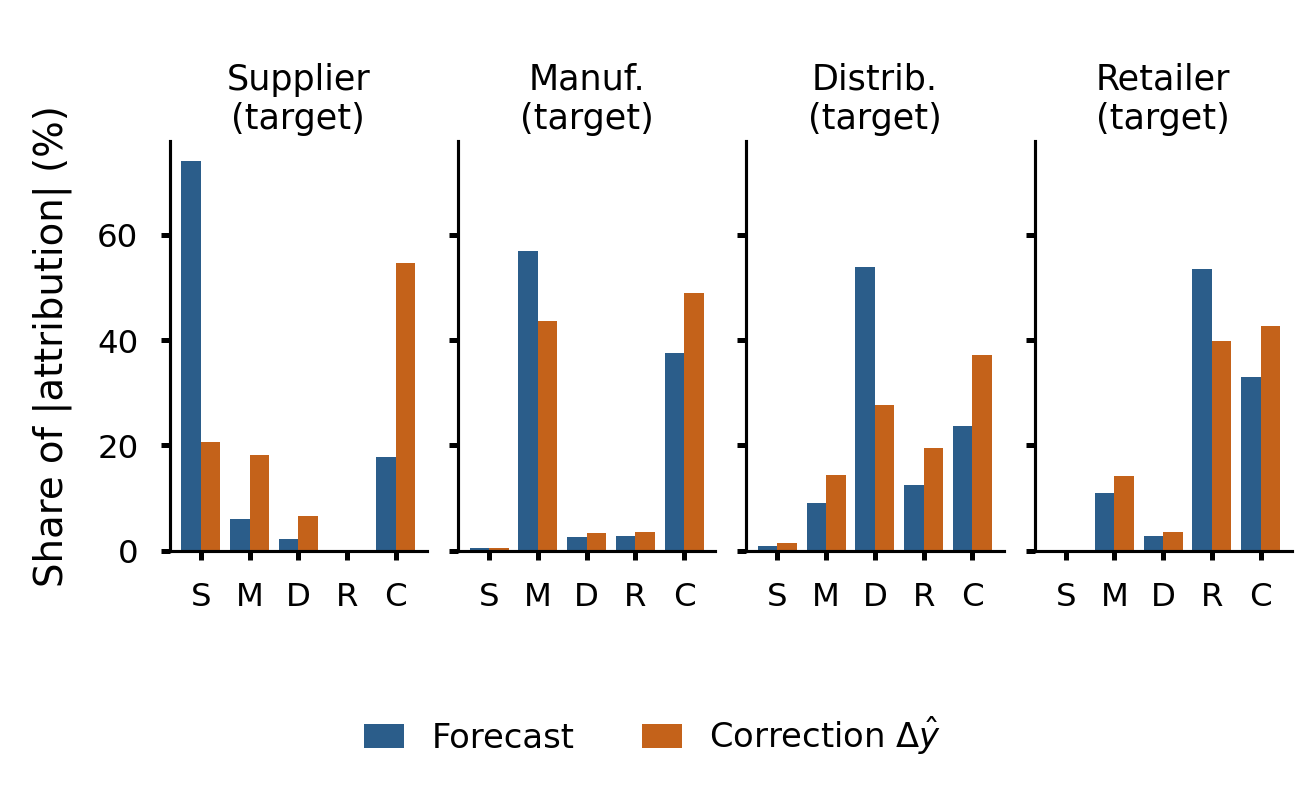
\includegraphics[width=\columnwidth]{fig7.png}
\caption{Share of $|$Integrated Gradients attribution$|$ by input (S, M, D, R: risk indices; C: Total Cost) for each target node, for the forecast (blue) and for the learned correction (orange); 100 test windows $\times$ 5 seeds.}
\label{fig:ig}
\end{figure}

\begin{table}[t]
\caption{Integrated Gradients Fidelity Checks}
\label{tab:ig}
\centering
\footnotesize
\begin{tabular}{@{}p{2.6cm}p{1.9cm}p{1.4cm}p{1.2cm}@{}}
\toprule
Check & Observed & Reference & Status \\
\midrule
Completeness gap $|\sum\mathrm{Attr}-\Delta f|$ (median / 95th pct / max; $n=2{,}000$) & $9.4\times10^{-5}$ / $3.1\times10^{-3}$ / $9.6\times10^{-2}$ & Ideal: 0 ($M=64$) & Small median, heavy tail \\
Deletion test: top-attributed vs random input (10 high-correction windows) & 7 of 10 pass & Top input should matter more than a random input & Windows selected for large corrections \\
Implementation invariance & Not tested & -- & Not verified \\
Attribution latency (CPU, one target, 64 steps) & about 36 ms & -- & Measured; varies between runs \\
\bottomrule
\end{tabular}
\end{table}

\subsection{Operational Use and Cautions}
\begin{itemize}
\item \textbf{Early warning on shock windows:} Because the gain over persistence is concentrated on shock windows, the forecast is most useful as a change detector, not as a continuous replacement for persistence.
\item \textbf{Node-level triage:} Four concurrent forecasts show which echelon is predicted to deteriorate; attributions show which inputs the model is sensitive to but do not establish cause.
\item \textbf{Alert quality:} On three-tier severity, persistence is more accurate than the learned models in our evaluation (83.6\% versus 81.3\%), so alert thresholds should be validated before operational use.
\end{itemize}

\subsection{Threats to Validity and Technical Limitations}
We identify the following limitations. (1) Only one linear four-echelon topology (S$\to$M$\to$D$\to$R) is evaluated. (2) The data are offline records from a single dataset, with no 2017 records. (3) Gradient attributions indicate sensitivity, not causal effects. (4) The graph-free LSTM differs from the ST-GCN in more than the graph, and a control with the same architecture and an identity adjacency was not run. (5) Severity tiers are defined by per-node terciles; the Supplier's tiers are very narrow. (6) The symmetric variant was unstable across seeds. (7) Results use one chronological split, with test data from Sep--Dec 2018. (8) The horizon is five rows, which is not always exactly ten minutes. (9) The deletion test was run on ten windows selected for large corrections, not on a random sample.

%==================================================================================
\section{Conclusion and Future Scope}
\subsection{Conclusion}
We presented SupplyGuard, a spatio-temporal model that forecasts the risk indices of four supply chain echelons concurrently. On the Mendeley SCRM dataset, the directed model reduced the mean-node MSE to $2.73\times10^{-4}$ ($R^2=0.973$), 31\% below Naive Persistence and 4\% below a graph-free LSTM, with the benefit concentrated on shock windows. Persistence, however, achieved higher three-tier severity accuracy, and the ablation is confounded, so we do not claim that graph structure alone explains the gain. Integrated Gradients attributions have a median completeness gap of $9.4\times10^{-5}$ with a heavy tail and describe the model's local sensitivity rather than causal effects; in our results each node's forecast is dominated by its own current value and the Total Cost, not by upstream echelons.

\subsection{Future Work}
\begin{itemize}
\item \textbf{Dynamic mesh topologies:} Extend to multi-supplier networks and test attention-based edge weights.
\item \textbf{External telemetry:} Add external signals such as weather or port congestion where data are available.
\item \textbf{Controlled ablation and hybrid alerts:} Run an identity-adjacency control with the same architecture, and test a hybrid that uses persistence in calm periods and the learned correction on detected shocks.
\end{itemize}

\section*{Acknowledgment}
The authors thank their project supervisor, Mrs.\ N.\ Chandana, Assistant Professor, Department of Computer Science and Engineering, Anurag University, Hyderabad, for her guidance throughout this work, and the authors of the Mendeley time-series dataset \cite{r3} for making it publicly available.

%==================================================================================
\begin{thebibliography}{20}
\bibitem{r1} D. Ivanov, A. Dolgui, and B. Sokolov, ``The impact of digital technology and Industry 4.0 on the ripple effect and supply chain risk analytics,'' \emph{Int. J. Prod. Res.}, 2018, doi: 10.1080/00207543.2018.1488086.
\bibitem{r2} D. Simchi-Levi, W. Schmidt, and Y. Wei, ``From superstorms to factory fires: Managing unpredictable supply-chain disruptions,'' \emph{Harvard Business Review}, vol. 92, no. 1--2, pp. 96--101, 2014.
\bibitem{r3} H. Banerjee, G. Saparia, V. Ganapathy, P. Garg, and V. M. Shenbagaraman, ``Time series dataset for risk assessment in supply chain networks,'' Mendeley Data, V2, 2019, doi: 10.17632/gystn6d3r4.2.
\bibitem{r4} S. Hochreiter and J. Schmidhuber, ``Long short-term memory,'' \emph{Neural Comput.}, vol. 9, no. 8, pp. 1735--1780, 1997, doi: 10.1162/neco.1997.9.8.1735.
\bibitem{r5} B. Yu, H. Yin, and Z. Zhu, ``Spatio-temporal graph convolutional networks: A deep learning framework for traffic forecasting,'' in \emph{Proc. 27th Int. Joint Conf. Artif. Intell. (IJCAI)}, 2018, pp. 3634--3640, doi: 10.24963/ijcai.2018/505.
\bibitem{r6} T. N. Kipf and M. Welling, ``Semi-supervised classification with graph convolutional networks,'' in \emph{Proc. 5th Int. Conf. Learn. Represent. (ICLR)}, 2017.
\bibitem{r7} A. Dolgui, D. Ivanov, and B. Sokolov, ``Ripple effect in the supply chain: An analysis and recent literature,'' \emph{Int. J. Prod. Res.}, vol. 56, no. 1--2, pp. 414--430, 2018, doi: 10.1080/00207543.2017.1387680.
\bibitem{r8} M. Sundararajan, A. Taly, and Q. Yan, ``Axiomatic attribution for deep networks,'' in \emph{Proc. 34th Int. Conf. Mach. Learn. (ICML)}, 2017, pp. 3319--3328.
\bibitem{r9} Z. Wu, S. Pan, F. Chen, G. Long, C. Zhang, and P. S. Yu, ``A comprehensive survey on graph neural networks,'' \emph{IEEE Trans. Neural Netw. Learn. Syst.}, vol. 32, no. 1, pp. 4--24, Jan. 2021, doi: 10.1109/TNNLS.2020.2978386.
\bibitem{r10} I. Farzhana and L. Dev Harris, ``Hybrid GNN-LSTM model for real-time supply chain risk prediction,'' in \emph{Proc. 8th Int. Conf. Comput. Methodologies Commun. (ICCMC)}, IEEE, 2025, doi: 10.1109/ICCMC65190.2025.11140739.
\bibitem{r11} F. Pedregosa \emph{et al.}, ``Scikit-learn: Machine learning in Python,'' \emph{J. Mach. Learn. Res.}, vol. 12, pp. 2825--2830, 2011.
\bibitem{r12} H. Min, ``Artificial intelligence in supply chain management: Theory and applications,'' \emph{Int. J. Logist. Res. Appl.}, vol. 13, no. 1, pp. 13--39, 2010.
\bibitem{r13} P. Veli\v{c}kovi\'c, G. Cucurull, A. Casanova, A. Romero, P. Li\`o, and Y. Bengio, ``Graph attention networks,'' in \emph{Proc. 6th Int. Conf. Learn. Represent. (ICLR)}, 2018.
\bibitem{r14} R. Caruana, ``Multitask learning,'' \emph{Mach. Learn.}, vol. 28, no. 1, pp. 41--75, 1997, doi: 10.1023/A:1007379606734.
\bibitem{r15} J. Adebayo, J. Gilmer, M. Muelly, I. Goodfellow, M. Hardt, and B. Kim, ``Sanity checks for saliency maps,'' in \emph{Proc. 32nd Conf. Neural Inf. Process. Syst. (NeurIPS)}, 2018, pp. 9505--9515.
\bibitem{r16} F. Scarselli, M. Gori, A. C. Tsoi, M. Hagenbuchner, and G. Monfardini, ``The graph neural network model,'' \emph{IEEE Trans. Neural Netw.}, vol. 20, no. 1, pp. 61--80, Jan. 2009.
\bibitem{r17} Y. Li, R. Yu, C. Shahabi, and Y. Liu, ``Diffusion convolutional recurrent neural network: Data-driven traffic forecasting,'' in \emph{Proc. 6th Int. Conf. Learn. Represent. (ICLR)}, 2018.
\bibitem{r18} K. He, X. Zhang, S. Ren, and J. Sun, ``Deep residual learning for image recognition,'' in \emph{Proc. IEEE Conf. Comput. Vis. Pattern Recognit. (CVPR)}, 2016, pp. 770--778.
\bibitem{r19} S. M. Lundberg and S.-I. Lee, ``A unified approach to interpreting model predictions,'' in \emph{Proc. 31st Conf. Neural Inf. Process. Syst. (NeurIPS)}, 2017, pp. 4765--4774.
\bibitem{r20} D. P. Kingma and J. Ba, ``Adam: A method for stochastic optimization,'' in \emph{Proc. 3rd Int. Conf. Learn. Represent. (ICLR)}, 2015.
\end{thebibliography}

\end{document}
